%
%   This file is derived from the APS files in the REVTeX 4 distribution.
%   Version 4.0 of REVTeX, August 2001
%
%   It has been simplified for use in Physics 3730/6720 by C. DeTar
%
%   Copyright (c) 2001 The American Physical Society.
%
%   See the REVTeX 4 README file for restrictions and more information.
%
% See the REVTeX 4 README file
%
\documentclass[aps,12pt]{revtex4}

\usepackage{graphicx}% Include figure files
\usepackage{bm}% bold math

\begin{document}

\title{Lab Exercise: LaTeX}

\author{Samir Suthar}

\affiliation{University of Utah, \linebreak Physics \& Astronomy Dept.}

\date{\today}

\maketitle

\section{In the Beginning...}
\label{sec:level1}

... there was light, and OH was it good!

\section{Math and Equations}
\begin{eqnarray}
\tan(\theta) = \mu/a \label{appa}
\\
\alpha = \sqrt{\beta^2 + \Lambda^2}
\\
w = y_2x_{15} + z_1^{2/3}
\\
\sigma^2 = \sum_{i=1}^N(x_i - \bar x)^2
\\
 x = \frac{-b \pm \sqrt{b^2 - 4ac}}{2a}
\\
z = \lim_{y \rightarrow \infty}f(y)
\end{eqnarray}

\begin{figure}[h]
\centerline{
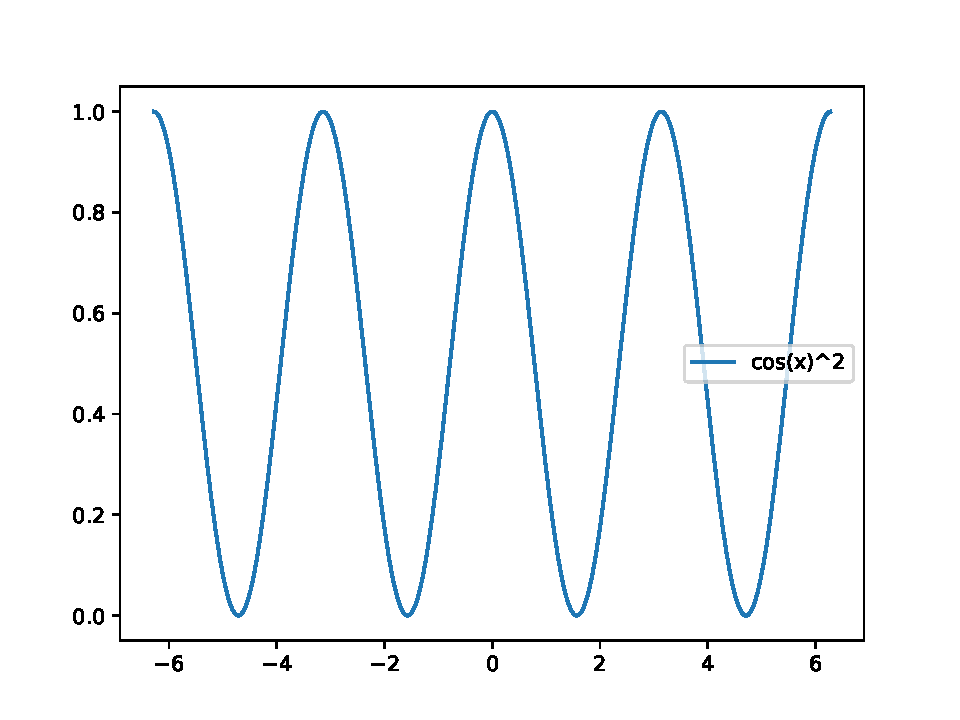
\includegraphics[width=4.5in]{cosX_sqr.pdf}
}
\caption{This is an arbitrary figure.}\label{fig:arb}
\end{figure}


\end{document}
